\chapter{Graph Databases using Neo4j}

Neo4j is a leading graph database that uses nodes, relationships, and properties to represent and store data. Unlike relational or document databases, Neo4j is optimized for highly connected data and complex queries involving relationships. It uses the Cypher query language for expressive graph traversals and pattern matching, making it ideal for applications with complex relationship structures and pathfinding requirements.

\section{Data Model and Setup}
For this task, we modeled a university system with three main entities: Students, Professors, and Courses. The relationships include:
\begin{itemize}
  \item \textbf{ENROLLED\_IN}: Connects a Student to a Course
  \item \textbf{TEACHES}: Connects a Professor to a Course
\end{itemize}

The data was loaded into Neo4j using Cypher scripts (see appendix for data details). The graph was visualized and queried using the Neo4j Browser.

\section{Graph Visualization}
Figure~\ref{fig:graph-visualization} shows the complete graph visualization of our university system. The graph displays:
\begin{itemize}
  \item \textbf{Pink nodes}: Students (Arjun Shrestha, Suraj Thapa, Sailesh Karki, Laxman Sharma)
  \item \textbf{Blue nodes}: Professors (Dr. Sita Devi, Dr. Ram Prasad)
  \item \textbf{Orange nodes}: Courses (Basic Electronics, Database Systems, Algorithms)
  \item \textbf{ENROLLED\_IN relationships}: Connect students to courses they are taking
  \item \textbf{TEACHES relationships}: Connect professors to courses they teach
\end{itemize}

This visualization clearly shows the interconnected nature of the university system, where Dr. Ram Prasad teaches both Algorithms and Database Systems, while Dr. Sita Devi teaches Basic Electronics. Students are enrolled in various courses, creating a web of relationships that can be efficiently queried using Cypher.

\begin{figure}[H]
  \centering
  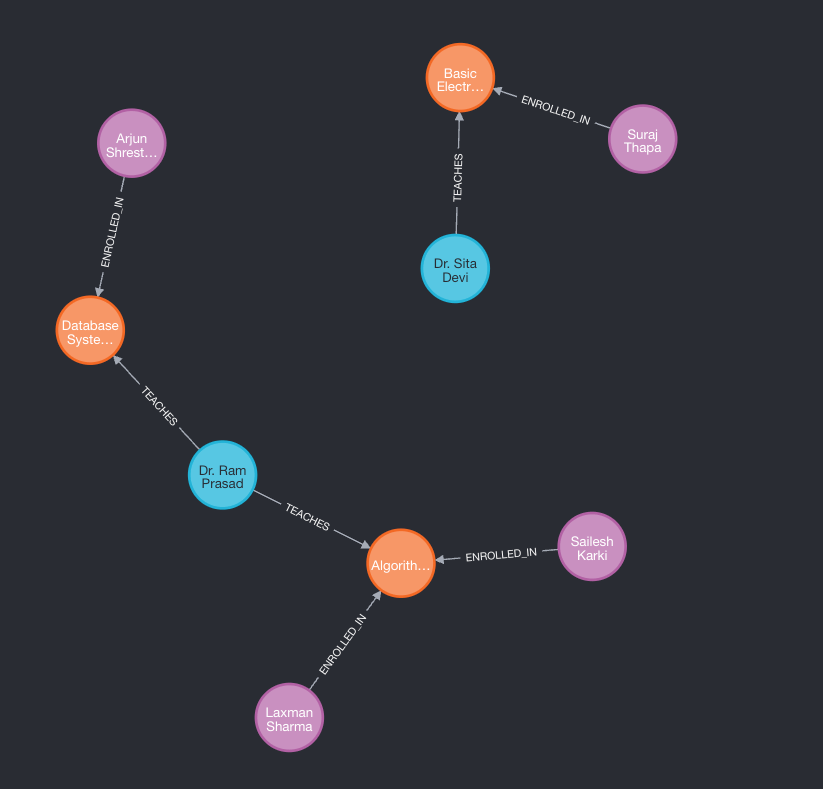
\includegraphics[width=0.9\textwidth]{task-3/screenshots/graph-visualization.png}
  \caption{Neo4j graph visualization showing the complete university system with students (pink), professors (blue), courses (orange), and their relationships.}
  \label{fig:graph-visualization}
\end{figure}

\section{Cypher Queries and Results}
Below, each Cypher query is briefly explained, followed by the result table and a reference to the corresponding screenshot in Appendix~B.

\subsection{All Professors and Their Courses}
\textbf{Query:}
\begin{minted}[fontsize=\small]{cypher}
MATCH (p:Professor)-[:TEACHES]->(c:Course)
RETURN p.name AS Professor, c.name AS Course
ORDER BY p.name, c.name;
\end{minted}
This query lists all professors and the courses they teach by traversing the TEACHES relationship.

\begin{table}[H]
  \centering
  \caption{All professors and their courses. See Appendix Figure~\ref{fig:task3-all-prof-courses}.}
  \begin{tabular}{ll}
    \textbf{Professor} & \textbf{Course} \\
    \hline
    \texttt{Dr. Ram Prasad} & \texttt{Algorithms} \\
    \texttt{Dr. Ram Prasad} & \texttt{Database Systems} \\
    \texttt{Dr. Sita Devi} & \texttt{Basic Electronics} \\
  \end{tabular}
\end{table}

\subsection{Courses by Prof. Ram Prasad}
\textbf{Query:}
\begin{minted}[fontsize=\small]{cypher}
MATCH (p:Professor {name: 'Dr. Ram Prasad'})-[:TEACHES]->(c:Course)
RETURN p.name AS Professor, c.name AS Course;
\end{minted}
This query finds all courses taught by Dr. Ram Prasad by filtering the professor node by name.

\begin{table}[H]
  \centering
  \caption{Courses taught by Dr. Ram Prasad. See Appendix Figure~\ref{fig:task3-courses-ram}.}
  \begin{tabular}{ll}
    \textbf{Professor} & \textbf{Course} \\
    \hline
    \texttt{Dr. Ram Prasad} & \texttt{Algorithms} \\
    \texttt{Dr. Ram Prasad} & \texttt{Database Systems} \\
  \end{tabular}
\end{table}

\subsection{Professors and Their Students}
\textbf{Query:}
\begin{minted}[fontsize=\small]{cypher}
MATCH (p:Professor)-[:TEACHES]->(c:Course)<-[:ENROLLED_IN]-(s:Student)
RETURN p.name AS Professor, c.name AS Course, s.name AS Student
ORDER BY Professor, Course, Student;
\end{minted}
This query finds all professors and their students by traversing from professors to courses they teach, and then to students enrolled in those courses.

\begin{table}[H]
  \centering
  \caption{Professors and their students. See Appendix Figure~\ref{fig:task3-prof-students}.}
  \begin{tabular}{lll}
    \textbf{Professor} & \textbf{Course} & \textbf{Student} \\
    \hline
    \texttt{Dr. Ram Prasad} & \texttt{Algorithms} & \texttt{Laxman Sharma} \\
    \texttt{Dr. Ram Prasad} & \texttt{Algorithms} & \texttt{Sailesh Karki} \\
    \texttt{Dr. Ram Prasad} & \texttt{Database Systems} & \texttt{Arjun Shrestha} \\
    \texttt{Dr. Sita Devi} & \texttt{Basic Electronics} & \texttt{Suraj Thapa} \\
  \end{tabular}
\end{table}

\subsection{All Students and Their Courses}
\textbf{Query:}
\begin{minted}[fontsize=\small]{cypher}
MATCH (s:Student)-[:ENROLLED_IN]->(c:Course)
RETURN s.name AS Student, c.name AS Course
ORDER BY s.name, c.name;
\end{minted}
This query lists all students and the courses they are enrolled in by traversing the ENROLLED\_IN relationship.

\begin{table}[H]
  \centering
  \caption{All students and their courses. See Appendix Figure~\ref{fig:task3-student-courses}.}
  \begin{tabular}{ll}
    \textbf{Student} & \textbf{Course} \\
    \hline
    \texttt{Arjun Shrestha} & \texttt{Database Systems} \\
    \texttt{Laxman Sharma} & \texttt{Algorithms} \\
    \texttt{Sailesh Karki} & \texttt{Algorithms} \\
    \texttt{Suraj Thapa} & \texttt{Basic Electronics} \\
  \end{tabular}
\end{table}

\subsection{Students in CS204}
\textbf{Query:}
\begin{minted}[fontsize=\small]{cypher}
MATCH (s:Student)-[:ENROLLED_IN]->(c:Course {code: 'CS204'})
RETURN s.name AS Student, c.name AS Course;
\end{minted}
This query finds all students enrolled in the course with code CS204 (Algorithms).

\begin{table}[H]
  \centering
  \caption{Students enrolled in CS204. See Appendix Figure~\ref{fig:task3-students-cs204}.}
  \begin{tabular}{ll}
    \textbf{Student} & \textbf{Course} \\
    \hline
    \texttt{Laxman Sharma} & \texttt{Algorithms} \\
    \texttt{Sailesh Karki} & \texttt{Algorithms} \\
  \end{tabular}
\end{table}

\subsection{Professors Who Teach More Than One Course}
\textbf{Query:}
\begin{minted}[fontsize=\small]{cypher}
MATCH (p:Professor)-[:TEACHES]->(c:Course)
WITH p, count(c) AS course_count
WHERE course_count > 1
RETURN p.name AS Professor, course_count
ORDER BY course_count DESC;
\end{minted}
This query finds professors who teach more than one course by counting the number of TEACHES relationships for each professor.

\begin{table}[H]
  \centering
  \caption{Professors who teach more than one course. See Appendix Figure~\ref{fig:task3-multi-course-prof}.}
  \begin{tabular}{lc}
    \textbf{Professor} & \textbf{Course Count} \\
    \hline
    \texttt{Dr. Ram Prasad} & \texttt{2} \\
  \end{tabular}
\end{table}

\subsection{Students Doing the Same Course}
\textbf{Query:}
\begin{minted}[fontsize=\small]{cypher}
MATCH (s1:Student)-[:ENROLLED_IN]->(c:Course)<-[:ENROLLED_IN]-(s2:Student)
WHERE s1.student_id < s2.student_id
RETURN c.name AS Course, s1.name AS Student1, s2.name AS Student2
ORDER BY Course, Student1, Student2;
\end{minted}
This query finds pairs of students who are enrolled in the same course.

\begin{table}[H]
  \centering
  \caption{Students doing the same course. See Appendix Figure~\ref{fig:task3-same-course}.}
  \begin{tabular}{lll}
    \textbf{Course} & \textbf{Student 1} & \textbf{Student 2} \\
    \hline
    \texttt{Algorithms} & \texttt{Laxman Sharma} & \texttt{Sailesh Karki} \\
  \end{tabular}
\end{table}

\section{Performance Analysis}

The Neo4j implementation demonstrated several key performance characteristics. The complete source code and implementation can be found at: \url{https://github.com/saileshbro/newsql-comparision.git/tree/main/task-3/data.cypher}.

\begin{itemize}
    \item \textbf{Relationship Traversal}: Queries involving relationship traversal showed excellent performance, especially for complex multi-hop queries
    \item \textbf{Pattern Matching}: Cypher's pattern matching capabilities enabled efficient querying of complex relationship structures
    \item \textbf{Graph Visualization}: The built-in visualization tools provided immediate insights into data relationships
    \item \textbf{Query Expressiveness}: Cypher queries were highly readable and expressive for complex graph operations
    \item \textbf{Index Performance}: Node and relationship indexes provided fast access to specific entities
\end{itemize}

\section{Use Cases and Applications}

Neo4j's graph database architecture makes it particularly suitable for:

\begin{itemize}
    \item \textbf{Social Networks}: Efficient storage and querying of user relationships and connections
    \item \textbf{Fraud Detection}: Pattern matching across complex relationship networks to identify suspicious activities
    \item \textbf{Knowledge Graphs}: Representing and querying complex knowledge structures and relationships
    \item \textbf{Recommendation Systems}: Traversing user-item relationships to generate personalized recommendations
    \item \textbf{Network Analysis}: Analyzing connectivity patterns and identifying influential nodes in networks
\end{itemize}

The university relationship modeling implementation demonstrates how Neo4j excels at handling complex interconnected data with natural relationship representation, powerful traversal capabilities, and intuitive query language, making it ideal for applications requiring deep relationship analysis and pattern recognition.